\Chapter{The Women of the Family}{Clare Court}

Now that we have reached this stage in our narration, readers will have observed that most of the characters who figure so prominently in this book are men, but I hasten to assure them that this is not intended to prove anything in particular. In an age when the liberation of women has become a subject which regularly hits the headlines, it seems only fair to pay some tribute to the female members of the family who for generations, worked away behind the scenes performing all the monotonous chores which enabled the menfolk to make full use of their own talent. There is little doubt that their personalities and intelligence had a very strong influence in the work of the family as a whole. There were of course sisters, cousins and aunts too numerous to mention individually, but I feel it worth recording something of the lives of the two women whom I actually met and came to know the best - William's sister Selina, and his wife Ada, my mother-in-law. Their names crop up frequently in the story and their influence (on William) probably stronger than any of the others.

The first and most obvious fact on which I feel qualified to pontificate is that any woman who becomes a Court by birth or marriage, need not expect an easy life. Interesting maybe, rewarding, demanding, varied - yes, certainly, and if my own experience is anything to go by, continually fraught with the problems brought about by combining a public life with an insufficient income. Looking back over the family history for the last seventy years and probably longer, one sustaining factor is very obvious - that the women considered it was their mission in life to smooth the path for the men in whatever projects they were engaged. Grandfather William Court, for example, spent much of his life working for the Temperance Cause and was a well-known figure in the area as he travelled from village to village on his white pony in order to speak at meetings. On Sundays, the pony bore him to preaching appointments, while at election time he was to be seen covering the same ground in the Liberal cause. As his wife was a semi-invalid, perhaps it was fortunate that he was so well provided with daughters - three altogether, who naturally enough took great pride in their father's activities and attended to all his wants.

When Grandfather died, the mantle of family responsibility descended to William, the second son (Lewis, the eldest having entered the ministry and left home). Two of William's sisters, Selina and Lily, had lost their husbands and were therefore constantly available. The third sister, Tilly, was unmarried and kept house for him until her death. It is hardly surprising to record that William was hopelessly spoilt by his sisters, particularly by Tilly. They had always been a close-knit family and William and Tilly understood each other particularly well. When poor Tilly died at the early age of forty, William was jolted out of his comfortable and well-regulated bachelor existence and it was probably this as much as anything which finally brought him to marry. So the patient Ada inherited the task of looking after William and always made it clear that she regarded this as a privilege. It is of course a firmly established country tradition to pamper the men of the house and I could point to several homes in our village where strict unwritten rules regarding the division of labour are still observed. While living in North Devon for ten years I came across many examples of this total dependence on the woman of the house, some of them very amusing to a bystander. One conversation which stays in the memory and was actually overheard between two young men:

\begin{quote}
\textbf{First Young Man}: Didn' see 'ee up the dance Friday night. \\
\textbf{Second Young Man}: No. \\ 
\textbf{First Young Man}: Why didn' 'ee cum then? \\
\textbf{Second Young Man}: Mother ad'n cleaned me shoes.
\end{quote}

\begin{figure}[]
	\centering
     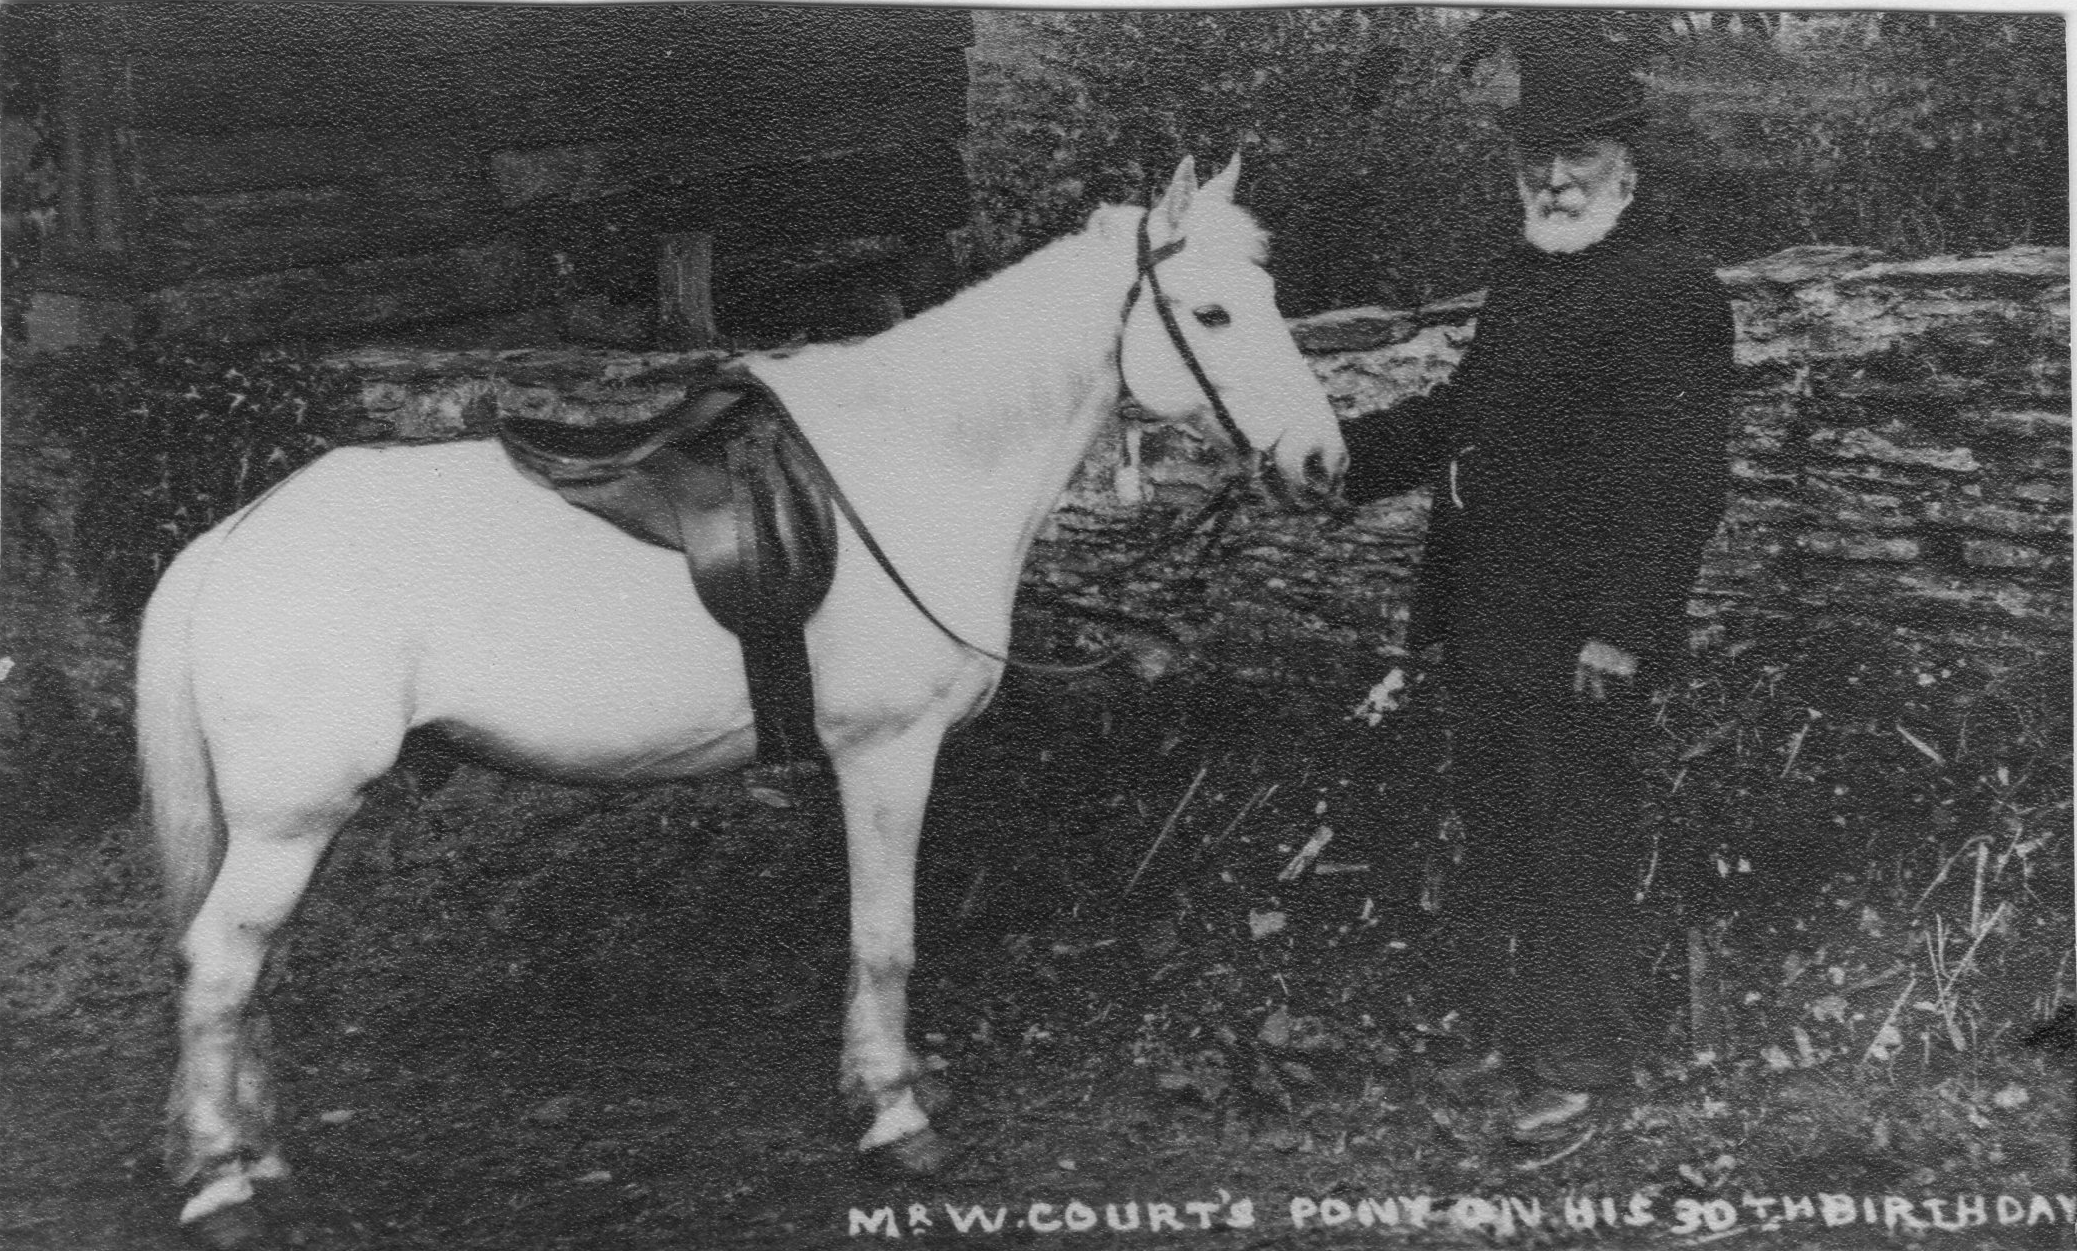
\includegraphics[width=1\textwidth]{figures/DapperPony}
     \caption{Grandfather William Court and his pony, Dapper}
     \label{fig:Pony}
\end{figure}



In the face of such telling argument, what remains to be said? \quotemark{Women's work}, however, an expression which must surely bring on apoplexy in ardent supporters of the Women's Liberation Movement, was not necessarily a derogatory phrase. It was the allotted share of the toil of daily living, accepted by women as an essential part of the pattern of life. For example, at Roadwater there were two houses, a Post Office and a family business to run, not counting activities connected with the Chapel, such as the preaching and Temperance Meetings. William with his sister Tilly and his father, (Grandfather), lived at Oatway House, also looking after the other old man, Grandfather Grinslade. The women's task was to look after the men, and to run the Post Office. William spent his days in the workshop dealing with the boots and bicycles and rarely if ever came into the shop. Great importance was attached to the men's preaching and everything possible was done to ensure that they were able to do the necessary study and preparation for this work. The garden which stretched up from Oatway, was \quotemark{men's work} of course, though William always used to grumble about this and avoided it when he could. All the men were very helpless when faced with the simplest domestic task. When Glyn was born and William was left alone in the house for a while, he lived on bread and cheese for several days having no idea how to prepare anything else. Tending the fire was woman's work - here again, considerable labour was involved as there was no proper storage space for fuel at Roadwater and logs and coal had to be brought some distance to the house. Ada rarely complained, but years later occasionally even she did raise her voice at William's reluctance to have anything to do with fetching coal and making up the fire. I recall a characteristic little episode which took place in about 1951.

My husband's parents were seated cosily by the fire while Glyn and I fitted in as well as we could around the rather large table that dominated the room. As frequently used to happen, Ada was dozing off in her chair; and the fire was getting a little low. She had already left some coal in the grate ready for this moment, but it never seemed to occur to William that he might be able to put it on himself. Instead, his voice was heard - \quotemark{Fire wants mending, Adie}! Adie dutifully complied, but I was glad that she had the spirit to register a mild protest at being roused from her chair after a long day which had begun at five o-clock. She was, after all, in her middle sixties. But it takes a long time to change a countryman's habits and Ada was not the woman to instigate a confrontation.

Anything in the nature of preparing food, shopping, washing and wiping dishes - all this was a field which was completely unknown to the men of the family. Over a long period of time, as in all businesses, there were periods of relative prosperity and periods of depression. In the prosperous times there was plenty of help available and the necessity for a helping hand was not quite so pressing. Grandfather always had a married couple living in at Oatway - the husband assisted with the business of cutting out and making the boots, while the wife helped in the home, performing those tasks which we nowadays tend to minimise but which in those days were a major operation such as the week's washing. First of all the water had to be drawn, then carried to the copper in the washhouse, in the orchard. Kindling had to be prepared and dry wood brought to light under the copper. More tubs of water had to be filled for rinsing and scrubbing purposes. So without a woman to help, washing day was very hard labour. Besides, Grandmother was delicate and had to take to her bed at an early age. In more modern times, up to the end of the thirties, as I have written elsewhere, Glyn's parents always had at least two employees and often more working for them at Washford. There was always one man, and sometimes two, working out in the workshop at the boots, shoes and later bicycles. In the post office there was a girl at the switchboard and another doing the counter work. Then, of course, there were frequent arrivals and departures of the postmen and van drivers, not to mention the village baker whose business was also conducted on the premises. There was always a helping hand available when it was needed, and the \quotemark{girls} in the office frequently turned away from their duties to take a turn at looking after the child, a welcome distraction from routine. In later years, of course, help became much harder to obtain, and the supply of girls dwindled drastically. Their quality also dropped noticeably, as increasing opportunities for education creamed off the abler girls and sent them to grammar schools. Poor Ada was never able to understand this - changing time hit her very hard, and she gradually became burdened with more and more responsibility with less and less help and a smaller income. William worried about this a good deal and tried to ensure that she would have assistance after his death, but was too old and sick to be able to work out a satisfactory solution.

Thinking of the girls, one is led into trying to count up all those who passed into Ada’s care over the years. They came in all sorts' and sizes, mainly local, often very able, and tended to stay for years. When times improved sufficiently for Glyn's parents to take a short holiday the girls even slept at the house, answering the phone at all hours and balancing up the accounts at the weekend. Alas! However, even the best girl will marry and it was always a sad day when having trained a willing assistant and come to rely on her services, she left and had to be replaced by a raw recruit. Here again changing times made things more difficult to those who were accustomed to the old order, and it would no longer be taken for granted that the girl would do up the accounts before leaving on Saturday evening. Not so many years before she would not have expected to leave until they balanced, and more than one disconsolate boyfriend waited in vain on a Saturday to take his young lady to the pictures.

Often in after years, the young ladies who had since matured into homely married women, would come back to see Mrs Court, and \quotemark{the office} as it was always called, would ring with noisy laughter as the proud mother showed off her children and told all her news. After her departure, peace would descend once more, and Granny would shake her head and smile, and pass some mild comment. \quotemark{She always was like that! The office was always noisy when she worked here!}

As far as housework was concerned, the women of the family of course always did their own, and even though she had a large house to look after, Ada would not have dreamt of asking another woman to clean it for money. In fact even when she was growing old and infirm she found it very difficult to delegate the cleaning to the willing daily lady and never stopped apologising for not doing it herself.

Alas poor Ada! She dearly loved polishing the oak floors and panelling that William had made and felt deprived when she could no longer do this work. The polishing was a sort of consummation of all the long years they had spent building the house together, giving spiritual contact with its departed creator. It is easy to sneer at these pleasant old-fashioned ways but when one looks at the insecurity of society today one can perhaps appreciate the advantages of the system in which the men's and women's roles were clearly defined. Only today in the Sunday newspaper I have read a very serious and well-meaning article about the insecurity of so many partners in modern marriages brought about mainly by the increased status; liberty and earning power of women, with the subsequent feelings of inadequacy which such independence induces among the males. Such problems were unknown to the generation of which I write, and although I for one would have no wish to return to those days, I still cannot repress a mild feeling of regret that while rejecting one role, women do not seem to have altogether succeeded in finding another which is satisfactory for the well-being of society as a whole.

When poverty lurks only just around the corner, there is little time for niceties and fanciful notions. Greatest and most dreaded ogre of all was the spectre of the Workhouse, Although times in the twenties and thirties were not quite as hard as they had been, there was still precious little money to waste, and no one could tell what lay in the future - so the safest and best way to insure oneself was to have a regular income, however small, from some modest investment. Cottages were cheap to buy, especially if purchased complete with tenant, and with a little renovation would often be improved sufficiently to bring in a higher rent than the accepted few shillings a week. One could hardly criticise William for failing to anticipate the effects of inflation. Already in his lifetime, the cottages were becoming a burden and had long since ceased to pay their way. When after the 1939 war, four cottages of Grandfather’s block at Watchet were demolished, the principal emotion was a heartfelt sense of relief.
 
\Flourish	 

My husband's mother, Ada Palser, was not a Somerset woman by birth but had been born hard by the shores of the Severn at Lydney in Gloucestershire. To the end of her life, although she rarely revisited her native town once she had left it, she was always a stout defender of the county; one of her favourite phrases, when the beauties of West Somerset were being described, was \quotemark{Mind you, there’s lovely country in Gloucestershire}. And very true, as many readers will no doubt agree.

Her father was a railwayman on the Great Western and the family lived in a four-roomed stone cottage by the side of the railway line just outside the town. The family name, Palser, is the same as Palliser, a fence-maker, but in her grandfather's time they had been farmers and millers at Wootton-under-Edge. Her mother's job, apart from looking after the family of six children, had been to open the crossing gate for trains to pass about five or six times of day. The lane past the cottage led down to Lydney's small but characterful harbour on the tidal Severn, now full of pleasure craft. We visited the spot a few years ago and spent a fascinating hour or two trying to relate the present reality with the past as it had so often been described to us. The cottage is no longer there but a happy chance, its appearance had been faithfully recorded by an enthusiastic amateur artist, who was only too pleased to make a copy of his picture for us. One tree in the orchard still survived, together with the remains of the pigsty. This little building was of some importance in the lives of the family as its occupants furnished additional protein for the family's diet, providing in addition to salt pork and brawn, meat for home-made faggots (the sage also grew in the garden) and pure lard to make lardy cakes with dough fetched from the baker. \quotemark{We lived well} she often used to say - \quotemark{My father earned twenty-eight shillings a week - that was good money in those days. We always had plenty to eat, and we could often pick up coal along the line. Oh yes, we were well off}.

Another of her recollections was of sitting on the steps of Lydney Cross waiting for Lord Bledisloe to drive past with his bride after his marriage in the early 1890’s.

When we revisited the crossing, the gate had been replaced, but only comparatively recently, by a more modern device - do-it-yourself model (captive wives no longer being readily available) has been installed. The lane from the harbour, past the cottage and into the town seemed remarkably unspoilt and cannot have changed very much since Ada’s childhood. As for the cottage itself, however, a heap of grey stones was all that was left - it had been demolished in order to improve visibility on the railway line.

When Ada was fourteen years old, her father was offered a better position with the G.W.R. in Swindon, and so the whole family prepared to move. Ada should have been leaving school by now but her mother was reluctant to send her to start an apprenticeship for such a short period as a year and allowed her to continue her education a little longer. So there she stayed, at the Church School in Lydney, a valued friend and assistant to the \quotemark{Governess} who taught her to work those elaborate and delicate crochet patterns in which she took so much delight.

On arrival in Swindon, Ada's employment could not be deferred any longer and it was here that she first entered the Post Office.

In her delightful book \quotemark{Lark Rise to Candleford} Flora Thompson describes her own humble beginnings in a village Post Office in Buckinghamshire. Much of this life she describes must have been almost as Ada knew it - though already, by 1901, there would have been slight changes. Flora Thompson, with the delicate observation of a true artist, notes the gradual alterations which were taking place in the decade, the 1880s. As Ada was born in 1884 she was only a few years later than this, and although village horizons were widening, there must have been many similarities. Flora Thompson describes how the hours of work in the Post Office were so loosely defined as to be almost permanent. Even Sundays was not sacred, as this was the day on which the Irish labourers used to come in to send their money home.

After starting work at Candleford, several months elapsed before Flora was even allowed to have a half day free in which to visit her mother. Commitment to work was expected to be total, though actual working conditions were probably relatively good in the Post Office. By the end of her life, Ada was so used to this that her whole life, waking and sleeping, coming and going, was completely ruled by the Post Office. Flora, as did Ada when she first came to Washford three years after starting her apprenticeship, received her board and lodging. Her spiritual, physical and moral welfare were under the close surveillance of a kindly mentor. Ada was similarly guarded, though her Miss Bellamy was noted for her sharp tongue. The work was far from unpleasant, involving as it did meeting all the folk of the surrounding district, writing letters or helping to compose telegrams for them. There was also a certain intellectual satisfaction in the deciphering of telegrams by Morse Code. Ada always enjoyed this and was well-known for reading the messages aloud as the buzzes came over the line. We still have the clock which was used to help in sending telegraph messages. It was not as efficient as a teleprinter perhaps, but infinitely more satisfying to use. Altogether life as a post office assistant was a very much happier lot than being tied to a factory bench in a Lancashire cotton mill, or permanently cooped up in the basement scullery of a large house. There was one gentleman's residence outside the village and the \quotemark{gentry} used to feature quite regularly in Ada's reminiscences. She had a respect for true gentility and courtesy, but could not abide \quotemark{jumped-up} parvenus.

During the period 1904-1920 Ada regularly attended the Methodist Chapel where she was a keen member of the choir and it was there that she met her future husband, William, also a Postmaster, at Roadwater. They postponed their marriage for years, as William was supporting a family of nephews and nieces, and, being well looked after by his unmarried sister, saw no particular urgency to change his situation. When he and Ada finally married in 1920, Ada was thirty-four and William forty-four. Many times he would joke in after years \quotemark{I'll never get married so young again}. But Ada regretted her late start. She would have liked to have had more children. Often, when struggling valiantly in her seventies with my energetic family of youngsters, she would laugh ruefully and say \quotemark{I ought to have been younger}.

Weddings are a time for sentiment and a time for gifts. Both of these were to be had in plenty and in particular a handsome marble clock from the people of the village. As for sentiment, not only was the list of subscribers to this gift recorded, but it has descended to us in its entirety. A glance at this list gives an interesting microcosm of village life at that time. At the head of the list stand Mr and Mrs Lysaght of Chapel Cleeve with a princely donation of two pounds each. This is an interesting sidelight on social change, as the Lysaghts had made their money in business and subsequently purchased the mansion of Cleeve where they remained for some thirty years, the house later becoming a hotel. Next came the Stoates - pillars of the prosperous farming community and faithful standard-bearers for Dissent since the 1790s. Next in size of donation come the gentry, the Leighs of Bardon. After that, nearly every farm and village family of the present day is represented. The good lady who collected all this money, largely in shillings and sixpences, is not known to us, but is none the less immortalised by her letter which is enclosed with the list of subscribers;

\begin{quote}
\textit{Dear Miss Palser. I hope you will understand this. I feels rather shakeing today, thank you ever so much miss for your letter I hope you can read this, if not, you must see the book, when you comes home, they are giving you a good present, and it will surprise you when you comes home I hear miss you are to be married next Tuesday, wish you the best of luck, and I hope miss you will have it nice and fine for the wedding. I have done all I could for you miss, and wish I could do more for you, will miss I suppose, if my man gets work he his in Bridgwater I am to be married soon, that is true miss, and miss Palser, miss Bellamy told me when you comes home, you was going to let me have a box, and miss if you will sell it to me. I should be please, as I can't afford to buy a new one, do you think miss you could let me have it the last week in this month as I shall be going away for a holiday. I would do anything for you. if you will be kind enought father as been out of work 4 weeks now makes me miserable. bad job for me. now miss if you cant unstand I will send you the book, your truly with Love M.Lewis.}
\end{quote}

And from a lady who evidently relished a touch of mystery:


\begin{quote}
\textit{Hearing when I was home last that you was collecting for a present for Miss Palser on account of her forthcoming marriage + leaving Washford P.0. (I have visited the P.0. for years) you will find my donation for £1.1.0 - one Guinea enclosed please use to that affect.}

from a well Wisher.
\end{quote}

A guinea indeed! More than the gentry! Who can she have been?

My mother-in-law was in her sixties when I first came to know her and one of the first things that struck me when I first came to Washford was how hard and long she worked every day of the week. Although the post office no longer held the important place that it once had in the area, it was still necessary to rise at an hour which seemed to me impossibly early in order to take in the morning mail. Her alarm clock, as I recall, was always set at ten past five. My father-in-law's health was failing, so in addition to their responsibility for all the post office work and caring for a sick husband, she had to deal increasingly with the shoe business as well. She never complained about this, and I was continually amazed at her capacity for endurance. She had inherited from her Gloucestershire forebears that stoicism tempered with simple humour which enabled them to bear the harshness of their existence. As she would have expressed it, \quotemark{tidn’t no good to complain, dear, is it?}

Though not at all demonstrative by nature Ada was a person of strong feeling and capable of deep affection and loyalty - especially to the family. Her particular weakness was for young children, and like many women of her generation she took great pleasure in spoiling her grandchildren. Not that she would have admitted it of course and each new gift of toys was accompanied by an apologetic \quotemark{We never had it}! The children of course took full advantage of this kindly figure with the silvery hair who rarely if ever scolded and could usually be relied upon for moral support when maternal favour was in short supply.

Ada loved to recall her own childhood. \quotemark{Mother was a good mother}, she would say, \quotemark{we were always well-dressed, and well fed, but we were afraid to go near her. The only time she praised us was when she was talking about us to other people - then there were no children like hers! But we never had the love}.

Starved of maternal affection in her youth she may have been, yet she amply made up for the lack in later life by lavishing her own on her nearest and dearest.

Growing up as she did in a working class home with few comforts and luxuries, she was accustomed to a more spartan style of living than her son and daughter-in-law. She rarely complained of the cold, and never in her life used a hot water bottle. Her appetite was also very moderate and she would often forget to eat for a day or so. Not that she begrudged spending money on food, for there was always an ample supply. \quotemark{I keep a good table}, she would say with justifiable pride. In fact I would frequently be alarmed at the quantities of food which I saw being put away in the larder, knowing full well that we could not possibly eat it all. Her tastes in food, based on old country ways of preserving with salt and vinegar, was different from mine, and it was at Washford that I first tasted pickled eggs and nasturtium seeds. Milk was always flowing in abundance, bread literally burst out of the bin. One of her little weaknesses was an inability to resist salesmen at the door, so that frequently she would buy a cake or loaf that she did not really want. She rarely bothered to see what she already had in the larder, so that like the shop new was put on top of old with rather alarming results. When we came to visit her we used to do our best to eat up what was fit for human consumption, this reducing the accumulation to manageable proportions - but to my horror I would find the next day that she would have bought three or four more large cakes, thinking that we would not have enough. And so it went on until after her death I came to turn out the larder properly. There was a sizeable bin, about the size of a small dustbin, full right to the top with packets of cake. We used what we could but the birds had the bulk.

I often wondered why she used to buy so much cake. It was almost as if the substance had a peculiar fascination for her, I surmise, perhaps erroneously, that it was for her a symbol of prosperity and affluence dating from childhood memories when cake was a rare and much prized speciality reserved only for treats and Sundays.

Ada was clever with her hands, a great lover of gardening and particularly talented with the knitting needle and crochet hook. In her younger days she spent most of her evenings working at crochet, and many and various are the pieces of work that she produced - table mats, edgings for tablecloths, in patterns of varied complexity. There were so many of these in the house that it seemed impossible to use them all, but I try to give each one a turn and very attractive they look when well starched and preseed. The quality of the cotton must have been excellent as they have withstood many a laundering with little sign of wear for nigh on seventy years.

One of these cloths has an interesting story and dates from her young days at Washford. Having become accustomed to seeing Ada constantly bent over her work crocheting during the evenings, James Bellamy rather light heartedly dared her to create a whole Biblical picture by this method - in short, to translate into slip stitch, chain, doubles and trebles the tale of Daniel in the Lion’s Den. The challenge was no doubt made in the same spirit in which an older man will dare a young woman to wield his spade or shoulder his heavy load, but Ada was not the woman to take such a challenge lightly. The idea appealed to her, and she stoutly maintained that she would tackle Daniel and his lions. Incredulous as only a man can be who knows little of such feminine matters, James Bellamy persisted in doubting her ability to fulfil the task and proceeded to set the seal on his incredulity by offering her a half sovereign if she really could achieve it. Ada set to work at once, and found the challenge a stimulating and absorbing one - so much so that she spent the whole of one winter's evenings not to mention a considerable number of balls of crochet cotton executing her design. At last she completed the cloth and worked a fringe to finish all off in the correct manner. But the half sovereign failed to materialise. James Bellamy had either forgotten his offer, or as seems more likely, changed his mind about parting with the money. After Ada's death, I found the cloth which had been put away for years and lost, though not the memories which went with it for I had often heard the tale. The tapestry (for it almost deserves the title though worked entirly in white cotton) is about the size of a small tablecloth. It depicts a heavily robed Daniel with prominent Jewish nose, recoiling from the brilliance of the angel's rays in the top right hand corner. Daniel perhaps is not completely convincing but one cannot fail to succumb to the charm of the two great bounding lions - one heavily bearded like a Victorian patriarch pretending to be very fierce, the other not even trying but very much enjoying having his likeness taken, like a modern television comic looking full at the camera. I imagine that Ada had copied the design from a picture in a book of Bible stories or perhaps from a family Bible.

Another hobby which never failed to delight her was dressing a doll, but as she was late marrying and did not have a little girl of her own to dress one for, William's nieces were the lucky recipients of her handiwork. Two of the dolls that she must have dressed in about 1910 survive almost intact and I have described them in the chapter about the museum.

In case I am making Ada seem like a plaster saint I must hasten to add that she had her little weaknesses. A strong streak of peasant obstinacy was probably one. (Her son finds his share very useful particularly in the political field.)

She did not really enjoy, as who indeed does, having her home disorganised by the invasion of children though loving the children themselves. Her religion was not of the spiritual order but strongly practical. I do not think she ever quite forgave God for taking William away from her - at any rate she stopped attending services after his death. She could be very disapproving, to the extent of being uncharitable, of certain people whom she disliked. Once dismissed to the doghouse, you were unlikely ever to be brought back into favour. One of her very forgivable little foibles was a love of bright sparkling gems and jewellery and she was rarely seen without one quite large ring, a splendid emerald set about with diamonds. Absent mindedness (and not due entirely to old age I am sure) frequently caused her to lose things, notably her spectacles, and no garden tool of hers would ever be found in its correct place. This trait also caused many a burnt dinner or ruined pudding - though she never missed the mail and only on very rare occasions was she not up to meet the postman at ten past six.

Before concluding this brief sketch of my husband's mother I must not forget to mention her love of music - particularly songs and choruses. As a girl, she had enjoyed the privilege of piano lessons. Her mother was very strict about practising and allowed no excuse, such as the icy coldness of the parlour, to prevent the daily half hour stint. Her teacher was a Miss Howells, sister of the composer and professor at the Royal College of Music, born in 1892, Herbert Howells. She remembered often seeing Herbert as a small child seated on the steps of the house as she passed along the street. Unfortunately she did not keep up her playing, but continuing her mother's tradition devoted her energy to ensuring that her own son practised every day. A curious and amusing little secret came out after her death. It transpired that when we were not at Washford, she would often sit at the piano and play some of the tunes she had learnt as a girl. She would also sing songs which she had learnt as a girl, sixty years before, complete with many verses. For some reason known only to herself, she did not want us to know that she played - though Glyn had sometimes found sheet music on the piano and had his suspicions. The children were quite hurt at this little deception which sprang, I am sure, from a harmless mixture of self-effacement and a tiny streak of obstinacy. She did enjoy a secret! Miss Bates, her assistant for the last few years, was often sorely tempted to tell us things we were not aware of, especially when Ada's health became worse, but so strong was my mother-in-law's personality that Miss Bates never dared to break the silence that had been enjoined upon her.

Ada's greatest friend and confidante in the immediate family and the only female member to venture far afield had been her sister-in-law, Selina. During the last decade of the nineteenth century, when jobs for working class girls were virtually unobtainable in her own area, Selina had sought employment as a lady's maid in \quotemark{gentlemen's houses}. Her first post was in the service of Bishop Moule at Cambridge. He was the author of several books of popular theology and also won a certain fame in his day as a hymn writer. Selina always spoke with warmth of the happy time she had spent in service at his house for the good Bishop's Christianity extended beyond the pulpit into the household, even to a shy maid with a Somerset accent. Perhaps he recognised intelligence when he saw it. At any rate, he would have been very surprised to learn how often his name was mentioned in that remote valley in Somerset for at least fifty years afterwards. From time to time, when visiting the relations at Roadwater, we would be shown a photograph dating from this period - it portrays a pale, serious girl most improbably garbed in academic dress. It appears that Selina had been dared by her fellow servants in the Cambridge house to don cap and gown and record the event for posterity. Accordingly she slipped off to the photographer on her afternoon off in order to have her picture taken. Anxious to escape detection, she walked right across Cambridge and sought out a photographer on the other side of the town. Imagine her chagrin and embarrassment at the service the following Sunday evening when, on placing her collection in the box, her eyes met those of the chapel steward -none other than the same photographer in his Sunday best! As far as has been recorded Selina’s scrape did not get her into trouble, but judging from the frequency with which she related the tale in after years, she had a lurking fear that the photographer's eye, like the judgment of Cain, would follow her to the tomb! Perhaps too she had a yearning for the academic life, as her education had been limited to a few years spent at the tiny Church School at Leighland. Be that as it may, the portrait does not convince despite a certain period charm, mainly because the aggressive pose and confident manner of the blue-stocking is lacking. There is something too about those large serious eyes, almost imploring \quotemark{Don't be cross with me - it's only a little joke}!

This happy employment lasted for several years until the Bishop won promotion which bore him away to the North, Selina was asked to accompany him but felt unwilling to go so far away from home.

She had never really felt at home in Cambridge despite the excellence of her situation, as she always used to say that the countryside was too flat, and that the climate affected her health. However that may be, she survived to the age of ninety-one so the bracing winds of East Anglia cannot have done her much harm after all. Her next situation was with the Rashleigh family at Menabilly near Fovey, and her work consisted of looking after the two young ladies of the family, Miss Rachel and Miss Kathleen. Many were the tales she used to tell of those days -the private path to the beach, exciting comings and goings of the gentry and of watching balls from the top of the staircase. The setting will be well known to readers of Daphne du Maurier, for she used it in her novels and the name Menabilly is thinly disguised as Mandalay. When her sight failed, Selina used to love to listen to radio versions of the du Maurier novels, and no doubt was able to offer many comments on the accuracy of the local colour. Only part of the year was spent at Menabilly, as the family also had a town house in Cumberland Terrace and thither they would all go to spend the winter.

After over fifteen years in service, Selina returned home to marry her Christopher who was a butler at a gentleman's house at Kingston St Mary near Taunton. Alas the marriage was short-lived and after only five years Christopher died of an undiagnosed illness - appendicitis perhaps, the cure for which was still its early stages.

Thenceforth, life became a long and tedious struggle and it was only with the help of the family that she was able to survive. She returned to Roadwater and took over the running of the Post Office, where she remained until her death over fifty years later. Towards the end of her life she lost her sight but right up to the end she never lost her charm and sense of humour. An expert needlewoman, she continued to sew until her sight prevented her. In appearance she was always scrupulously neat and despite her tiny income, well-dressed. Even at the age of ninety, I remember her sitting out of her bed attired in a pink dressing gown with a matching bow in her hair! While remembering her with affection, I regret that we had not been nearer in age. I feel that we should have had much in common.
